\section{Preliminaries}\label{Section:Preliminaries}

%BN, OOBN, Dynamic BN.
%Preliminaries for the temporal series data analysis: correlograms, partial correlograms. %Preliminaries for the AMIDST models.

\subsection{Dynamic Bayesian Networks}



\begin{figure}
\begin{center}
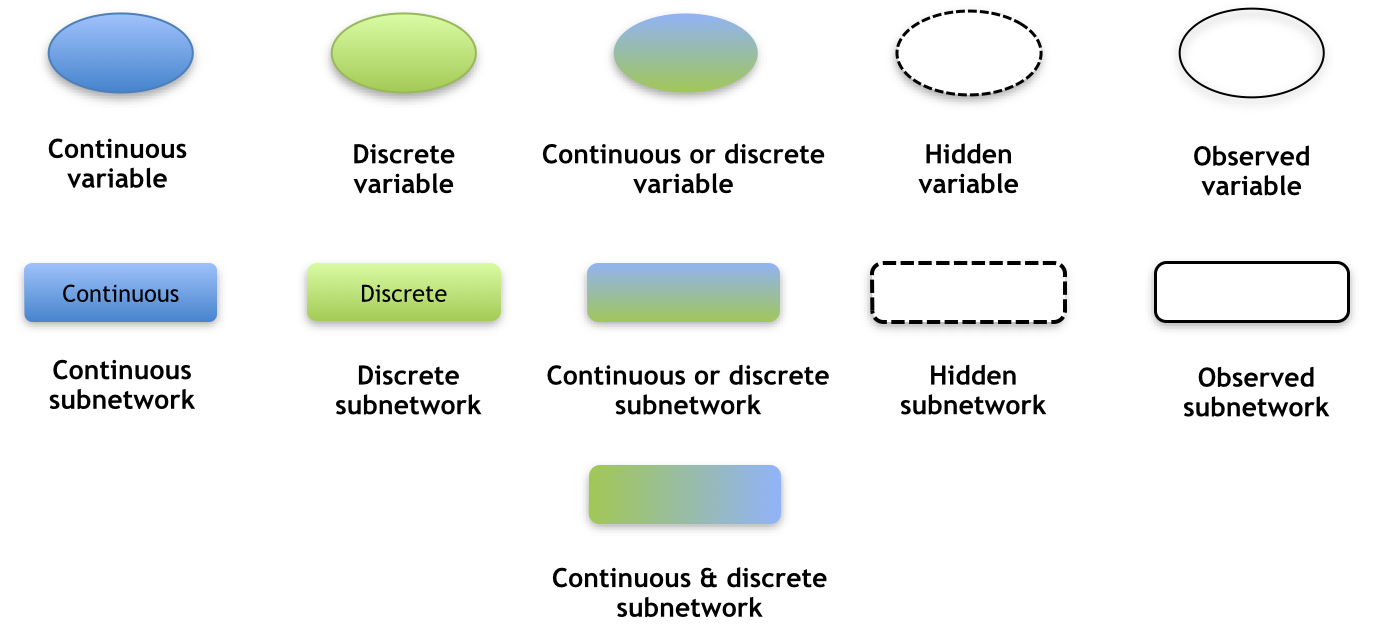
\includegraphics[scale=0.4]{./figures/PreliminariesNotation}
\caption{\label{Figure:PreliminariesNotation}PreliminariesNotation
}
\end{center}
\end{figure}





\subsection{Data Analysis}

As already commented in the introduction, the data analysis detailed here will be used to try to test some of the assumptions supporting the models elicited by the experts in the different use cases, but also to complement our understanding about the nature of the problem we are modelling. The set of tools employed for this purpose try to get insights about some simple and basic aspects of the structural and the distributional assumptions present in a dynamic Bayesian network.


\subsubsection*{Structural assumptions:  Correlograms and Partial Correlograms}

A DBN mainly tries to model complex multivariate time series. By using sample correlogramas and sample partial correlograms we will try to test if the available data support the temporal correlation between variables assumed by the DBN model, i.e. the temporal links between variables. However, these tools will only allow us to look at univariate time series, what strongly limits the validity of  conclusions. But, at least and as we will see in the different use-cases, this analysis will give us some interesting insights that are highly difficult to be elicited from experts.  


\begin{description}
\item[Sample Correlogram]:  Let ${x_1,...,x_T}$ be a univariate time series. The \emph{sample autocorrelation coefficient at lag v} is given by 

$$ \hat{\rho}_v =\frac{\sum_{t=1}^{T-v} (x_t-\bar{x})(x_{t+v}-\bar{x})}{\sum_{t=1}^{n} (x_t-\bar{x})^2}$$ 

\noindent $\bar{x}$ is the sample mean. The plot of $\hat{p}_v$ versus $v$ for $v=1,...,M$ for some maximum $M$ is called the \textbf{sample correlogram} of the data.



\item[Sample Partial Correlogram]: Let us denote by $X_t$ to the random variable associated to $X$ taking values at time $t$. We can build the following regression problem:

$$ X_t = a_0 + a_1X_{t-1} + a_2X_{t-2} + ... a_{v-1}X_{t-v-1}$$

Let us also denote $e_{i,v}$ to the residuals of this regression problem (i.e. the error when estimating $X_t$ using a linear combination of the $v-1$ previous observations). The \emph{sample partial autocorrelation coefficient of lag v}, denoted by  $\hat{\theta}_v$, is the the standard sample autocorrelation between  the variable $X_{t-v}$ and these residuals. Intuitively, the sample partial autocorrelation coefficient of lag v can be seen as the correlation between $X_t$ and $X_{t+v}$ after having removed the common \textbf{linear} effect of the data in between.

\end{description}

\subsubsection*{Distributional assumptions: Histograms and Bivariate Distributions}





For example, we are going to test whether



The aim of the analysis detailed in this section was the following. As commented in the introduction, the models presented from the different use cases were mainly built by expert knowledge. However, when defining these models we did not want to rely only on 


